\section{Algebra}

\subsection{Lineární algebra}

\begin{definition}[Vektorový prostor]
    Nechť $\mathbb{F}$ je pole
    a $V$ je množina vektorů dané délky nad tímto polem.
    $(\mathbb{F}, V, +, \cdot, 0, -, 1)$ nazveme {\em vektorový prostor}
    nad $\mathbb{F}$,
    pokud
    \begin{enumerate}
        \item $(V, +, 0, -)$ je komutativní grupa,
        \item násobení $\mathbb{F}$ a $V$ je kompatibilní
        ($a, b \in \mathbb{F}, \overline{v} \in V : a(b\overline{v}) = (ab)\overline{v}$),
        \item $1$ je identita pro $\cdot$,
        \item sčítání skalárů distribuuje přes násobení vektorem,
        \item sčítání vektorů distribuuje přes násobení skalárem.
    \end{enumerate}
\end{definition}

Vektor $u$ je {\em lineární kombinací} vektorů $v, w$, pokud existují
$a,b \in \mathbb{F}$ takové, že $u = av + bw$.
Množinu vektorů $M$ nazveme {\em lineárně nezávislou}, pokud žádný
vektor z~$M$ není lineární kombinací jiných vektorů z~$M$.

\begin{definition}[Báze prostoru]
    Nechť $\mathcal{V}$ je vektorový prostor.
    Množina vektorů $B = \{ b_i \}_{i \in I}$ je {\em báze} $\mathcal{V}$,
    pokud $B$ je lineárně nezávislá
    a každý vektor $v \in V$ lze vyjádřit jako lineární kombinaci
    vektorů z $B$.
\end{definition}

\begin{definition}[Dimenze]
    Dimenze prostoru je počet vektorů v~jeho bázi.
\end{definition}

\begin{definition}[Skalární součin]
    Nechť $u, v$ jsou vektory v~nějakém vektorovém prostoru.
    Skalární součin $u, v$ definujeme
    $u \cdot v = \sum u_i \cdot v_i$.
\end{definition}

Geometricky můžeme skalární součin definovat jako
$u \cdot v = \lvert u \rvert \cdot \lvert v \rvert \cdot \cos \theta$,
kde $\theta$ je úhel svíraný $u,v$. Zejména pak kolmé
vektory mají skalární součin 0, zatímco vektory se shodným směrem
mají skalární součin roven součinu jejich délek.

%\begin{definition}[Vektorový součin]

%\end{definition}

Nyní se zaměříme na matice. {\em Hodnost} (rank) matice je dimenze
prostoru generovaného jejími sloupci.

\begin{figure}[h]
    \centering
    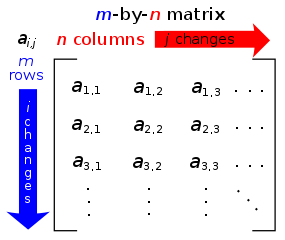
\includegraphics[width=120pt]{matrix.png}
    \caption{Matice a její rozměry, \href{https://commons.wikimedia.org/wiki/File:Matrix.svg}{zdroj}}
\end{figure}


\begin{definition}[Součin matic]
    Nechť $A$ je $n \times m$ matice a $B$ je $m \times p$ matice.
    Každá položka {\em součinu} $AB$ je zadána
    $(AB)_{ij} = \sum^{m}_{k = 1} A_{ik} B_{kj}$.
\end{definition}


Důležitou charakteristikou matice $A$ o rozměru $n \times n$ je {\em
determinant}, značený $\lvert A \rvert$. Geometricky se můžeme na matici
dívat jako vektory, které zadávají strany nějakého pravidelného
geometrického útvaru (třeba čtverce). Determinant je potom orientovaný
obsah tohoto obrazce.

Pro výpočet determinantu malých matic ($2\times2,
3\times3$) použijeme většinou Sarrusovo pravidlo (součet součinu
protažených levých diagonál mínus součet součinu protažených pravých
diagonál), pro větší
Laplaceův rozvoj.

Laplaceův rozvoj je výpočet založený na tom, že zafixujeme nějaký řádek
$i$ či sloupec $j$ (zejména se hodí takové, kde se vyskytuje hodně nul)
a pak použijeme
\[
    \lvert A \rvert
    = \sum_{j' = 1}^{n} a_{ij'} (-1)^{i + j'} M_{ij'}
    = \sum_{i' = 1}^{n} a_{i'j} (-1)^{i' + j} M_{i'j}
\]
kde $M_{ij}$ je determinant matice $A$ po odstranění řádku $i$ a sloupce
$j$.


\begin{definition}
    Nechť $A$ je $n \times n$ matice. Matici $B$ nazveme
    {\em inverzí k}~$A$, pokud $AB = BA = I_n$.

    Pokud existuje pro matici $A$ inverze, nazýváme $A$
    {\em invertibilní}.
\end{definition}

\begin{example}
    Matice níže není invertibilní.
    \[
        \begin{pmatrix}
            1 & 0 \\
            0 & 0
        \end{pmatrix}
    \]
\end{example}

Matice je invertibilní právě tehdy, když její determinant je různý od
nuly. Pro inverze $2 \times 2$ matic máme jednoduchý vzorec

    \[
        \begin{pmatrix}
            a & b \\
            c & d
        \end{pmatrix}^{-1}
        =
        \frac{1}{ad - cd}
        \begin{pmatrix}
            d & -b \\
            -c & c
        \end{pmatrix}
    \]
Větší matice zapíšeme ve tvaru $(A \mid I)$, upravíme $A$ na $I$, čímž
na pravé straně získáme inverzi k $A$.

\begin{definition}
    Matici $(a_{i,j})$ nazveme {\em diagonální} pokud
    \[ a_{i,j} \neq 0 \implies i = j \]
    Matici $A$ nazveme {\em diagonalizovatelnou} pokud existuje matice
    $P$ taková, že \linebreak $P^{-1} A P$ je diagonální.
\end{definition}

Máme-li tedy pro diagonalizovatelnou matici $A$ odpovídající diagonální
matici $D = P^{-1} A P$, potom platí, že $A = P D P^{-1}$, čímž se
dostáváme k~hlavní aplikaci: $A^k = P D^k P^{-1}$.

Platí podmínka, že pokud má $n \times n$ matice právě $n$ různých
vlastních čísel, potom je diagonalizovatelná. Pozor, nejedná se o
ekvivalenci.

Zbývá zjistit, jak matice diagonalizovat.
Pro danou matici $A$, získáme matici $P$ jako
soubor vlastních vektorů $A$. Diagonální matice
$D = P^{-1} A P$ je tvořena vlastními čísly $A$.

\begin{definition}
    Nechť $A$ je matice, $v$ nenulový vektor a $\lambda$ číslo.
    Pokud platí $A v = \lambda v$, potom $v$ nazveme {\em vlastní
    vektor} a $\lambda$ jemu příslušné {\em vlastní číslo}.
\end{definition}

Vlastní čísla jsou řešení {\em charakteristické rovnice} matice $A$,
která je zadána jako determinant $A - \lambda I$ (kde $\lambda$ je
proměnná).
Se znalostí vlastních čísel najdeme vlastní vektory jako řešení rovnice
$(A - \lambda I) v = 0$ (kde $\lambda$ je pevně zvolené vlastní číslo).

\subsection{Grupy, okruhy a pole}

Pojmy jsou zavedeny pomocí jazyka univerzální algebry. V celé podsekci
nechť $A$ je množina, $\cdot$ a $+$ jsou binární, $1$ a $0$ jsou
nulární, ${^{-1}}$ a $-$ jsou unární operace.

\begin{definition}[Pologrupa]
    Algebra $(A, \cdot)$ je {\em pologrupa},
    pokud splňuje rovnost
    $(x \cdot y) \cdot z = x \cdot (y \cdot z)$.
\end{definition}

Příkladem pologrupy je libovolná množina seznamů s~operací zřetězení
nebo množina matic s operací násobení.

\begin{definition}[Monoid]
    Algebra $(A, \cdot, 1)$ je {\em monoid}, pokud
    splňuje rovnosti
    $(x \cdot y) \cdot z = x \cdot (y \cdot z)$,
    $1 \cdot x = x = x \cdot 1$.
\end{definition}

Příkladem monoidu je množina všech seznamů s~operací zřetězení nebo
množina celých čísel s~operací sčítání.

V~každém monoidu $(A, \cdot, 1)$ existuje pouze jeden neutrální
prvek. Pro důkaz předpokládejme, že existuje nějaký neutrální prvek $1'$.
Potom $1 = 1 \cdot 1' = 1'$.

\begin{definition}[Grupa]
    Algebra $(A, \cdot, 1, {^{-1}})$ je grupa, pokud
    je $(A, \cdot)$ monoid a splňuje rovnost $a \cdot a^{-1} = 1 = a^{-1} \cdot a$.
\end{definition}

Například $(\mathbb{Z}, +, -)$ tvoří grupu (kde $-$ je unární).
Také $(\mathbb{Z}^*_n, \cdot, {^{-1}})$ pro dané $n \in \mathbb{N}$ tvoří grupu.

V~každé grupě $(G, \cdot, {^{-1}})$ existuje pro každé $g \in G$ nejvýše
(a tedy právě) jeden inverzní prvek.
Pro důkaz nechť $g$ má oboustranné inverze $x,y$.
Potom $x = x \cdot e = x \cdot (g \cdot y) = (g \cdot x) \cdot y
= e \cdot y = y$, stejně tak v~případě opačné strany
($x = e \cdot x = (y \cdot g) \cdot x =\ldots$),
tedy $x = y$. V~důkazu jsme použili pouze asociativity a neutrálního
prvku, důkaz existence nejvýše jedné inverze platí tedy i pro monoid.


\begin{definition}[Okruh]
    Algebra $(A, +, \cdot, 0, 1, -)$ je {\em okruh}, pokud
    $(A, +, 0, -)$ je komutativní grupa
    a $(A, \cdot, 1)$ je monoid
    a navíc splňuje distributivní rovnosti
    $a \cdot (b + c) = (a \cdot b) + (a \cdot c)$,
    $(b + c) \cdot a = (b \cdot a) + (c \cdot a)$.

    Okruh nazveme komutativním, pokud $(A, \cdot, 1)$ je komutativní.
\end{definition}

\begin{example}
    $(\mathbb{R}, +, \cdot, 0, 1, -)$
\end{example}

\begin{example}
$(\mathbb{R}[x], +, \cdot, 0, 1, -)$.
\end{example}

\begin{example}
    Množina $2 \times 2$ reálných matic s~běžnými operacemi.
\end{example}

V~okruhu platí vlastnosti, které dědí z~příslušné grupy a monoidu.
Navíc například v~okruhu platí, že 0 = 1 právě když je triviální (jeden
směr je zřejmý, v~druhém $a = 1 \cdot a = 0 \cdot a = 0$ pro lib. $a$).

\begin{definition}
    Nechť $R$ je okruh.
    $\emptyset \neq I \subseteq R$ nazveme {\em levý ideál} v~$R$
    pokud pro každé $x,y \in I$ a $r \in R$ platí
    $x + y, rx \in I$.
\end{definition}

\begin{example}
    Nechť $R = \mathbb{Z}_2[x] / (x^n - 1)$ je okruh polynomů
    a $C$ je nějaký cyklický kód zadaný polynomy v~$R$.
    Potom $C$ je ideál v~$R$.
    $C$ je dokonce {\em hlavní ideál}, což je ideál generovaný jediným prvkem.
\end{example}

\begin{definition}
    {\em Obor integrity} nazveme okruh $\mathcal{R}$, ve kterém platí
    \[
        \forall a,b \in R, a \neq 0, b \neq 0, a \cdot b \neq 0
    \]
\end{definition}


\begin{definition}[Pole]
Komutativní okruh $(A, +, \cdot, 0, 1, -)$ nazveme {\em pole}, pokud
pro každé $a \neq 0$ existuje $a^{-1}$ takové, že $a \cdot a^{-1} = 1$.
\end{definition}

\begin{example}
    $\mathbb{Q}, \mathbb{R}, \mathbb{C}, \mathbb{Z}_n.$
\end{example}

Každé pole je obor integrity. Pole již nelze zadefinovat rovnostmi.

\subsection{Teorie svazů}

\begin{definition}[Supremum]
    Nechť $(A, \leq)$ je částečně uspořádaná množina
    a $K \subseteq A$. Pokud existuje prvek $\bigvee K \in A$ takový,
    že
    \begin{itemize}
        \item je horní závora ($\forall k \in K . k \leq \bigvee K$)
        \item a je z horních závor nejmenší
    ($\forall c \in A, k \in K . k \leq c \implies \bigvee K \leq c$),
    \end{itemize}
    pak jej nazveme {\em supremum}.
\end{definition}

\begin{definition}[Polosvaz]
    $(A, \vee)$ nazveme {\em polosvaz}, je-li to komutativní a
    idempotentní pologrupa.

    Stejně tak částečně uspořádanou množinu $(A, \leq)$ nazveme
    {\em polosvaz}, pokud pro každou dvouprvkovou podmnožinu existuje supremum.
\end{definition}

Výše uvedené definice jsou ekvivalentní, v~jednom směru platí
$a \leq b \iff a \vee b = b$, v druhém se tak uspořádání definuje.

\begin{definition}[Svaz]
    $(A, \vee, \wedge)$ nazveme {\em svaz}, jsou-li
    $(A, \vee)$, $(A, \wedge)$ polosvazy a navíc platí absorpční zákony,
    tedy pro každé $a, b$
    \[ a \vee (a \wedge b) = a \wedge (a \vee b) = a \]

    Stejně tak částečně uspořádanou množinu $(A, \leq)$ nazveme
    {\em svaz}, pokud pro každou dvouprvkovou podmnožinu existuje
    supremum i infimum.
\end{definition}

Opět platí, že obě definice jsou ekvivalentní.

\begin{figure}[h!]
\centering
\begin{tikzpicture}
    \node[dot] (1) at (0,1) {};
    \node[dot] (a) at (-0.5,0) {};
    \node[dot] (b) at (0.5,0) {};
    \node[dot] (0) at (0,-1) {};
    \draw
        (1) -- (a)
        (1) -- (b)
        (0) -- (a)
        (0) -- (b);
\end{tikzpicture}
\hspace{10pt}
\begin{tikzpicture}
    \node[dot] (a) at (0,0) {};
    \node[dot] (b) at (1,0) {};
    \node[dot] (c) at (0,1) {};
    \node[dot] (d) at (1,1) {};
    \draw
        (a) -- (c)
        (a) -- (d)
        (b) -- (c)
        (b) -- (d);
\end{tikzpicture}
\hspace{10pt}
\begin{tikzpicture}
    \node[dot] (-1) at (0,0) {};
    \node[dot] (-2) at (0,-0.7) {};
    \node[dot] (-almostinf) at (0,-1.4) {};
    \node[dot] (-inf) at (-0.5,-2.1) {};
    \node[dot] (-inff) at (0.5,-2.1) {};
    \draw
        (-1) -- (-2)
        (-almostinf) -- (-inf)
        (-almostinf) -- (-inff);

    \draw[dotted]
        (-2) -- (-almostinf);
\end{tikzpicture}
\caption{
Příklad svazu a dvou uspořádaných množin, které nejsou svazy.}
\end{figure}

Pojmy morfismů algebraicky definovaných svazů získáváme
z~pojmu homomorfismus (zachovává výsledky operací)
a izomorfismus (bijektivní homomorfismus) algeber. Navíc zavedeme pojmy
izomorfismu svazů jakožto částečně uspořádaných množin se supremy a infimy.

\begin{definition}[Izomorfismus svazů]
    Zobrazení $\varphi : A \to B$ částečně uspořádaných množin
    $(A, \leq)$, $(B, \prec)$ nazveme {\em izotonní},
    pokud $a \leq b \implies \varphi(a) \prec \varphi(b)$.
    Bijekce $\varphi : L \to M$ je izomorfismus svazů
    $(L, \leq)$ a $(M, \prec)$, pokud $\varphi$ i $\varphi^{-1}$ jsou
    izotonní.
\end{definition}

\begin{figure}[h!]
\centering
\begin{tikzpicture}
    \node[dot] (a) at (0.5,-0.5) {};
    \node[dot] (b) at (0,0) {};
    \node[dot] (c) at (1,0) {};
    \node[dot] (d) at (0.5,0.5) {};


    \node[dot] (0) at (2, -0.75) {};
    \node[dot] (1) at (2, -0.25) {};
    \node[dot] (2) at (2, 0.25) {};
    \node[dot] (3) at (2, 0.75) {};
    \draw
        (a) -- (b)
        (a) -- (c)
        (b) -- (d)
        (c) -- (d)
        (0) -- (1)
        (1) -- (2)
        (2) -- (3)
        ;
    \draw[dashed, ->] (a) -- (0);
    \draw[dashed, ->] (b) -- (1);
    \draw[dashed, ->] (c) -- (2);
    \draw[dashed, ->] (d) -- (3);
\end{tikzpicture}
\caption{Izotonní zobrazení, které není izomorfismus (ani homomorfismus).}
\end{figure}

\begin{claim}
    Obě definice izomorfismů jsou ekvivalentní.
\end{claim}

\begin{definition}[Úplný svaz]
    Nechť $(L, \leq)$ je částečně uspořádaná množina.
    $L$ nazveme {\em úplný svaz} pokud pro každou (i prázdnou)
    $K \subseteq L$ existuje infimum i supremum.
\end{definition}

Infimum prázdné množiny je největší prvek v~uspořádání,
zatímco supremum prázdné množiny je nejmenší prvek v~uspořádání.

\begin{note}
    Každý konečný svaz je úplný, s~výjimkou prázdného.
\end{note}

Následující tvrzení dává užitečnou charakterizaci pomocí jediné
podmínky.

\begin{claim}
    $(L, \leq)$ je úplný svaz právě tehdy, když pro každou podmnožinu
    existuje infimum, právě tehdy, když pro každou podmnožinu existuje
    supremum.
\end{claim}

V~praxi informatiky je důležité následující tvrzení o pevných bodech.

\begin{claim}[Knaster-Tarski]
    Nechť $(L, \leq)$ je úplný svaz a $\varphi : L \to L$ je izotonní
    zobrazení,
    potom množina pevných bodů $\varphi$ tvoří úplný svaz.
\end{claim}

\pagebreak

Pro další podsekce budeme potřebovat následující dva svazy.

\begin{figure}[h!]
\centering
\begin{tikzpicture}
    \node[dot] (1) at (0,1) {};
    \node[dot, label=left:${a \wedge (b \vee c) = a}$] (a) at (-1,0) {};
    \node[dot, label=right:$b$] (b) at (0,0) {};
    \node[dot, label=right:$c$] (c) at (1,0) {};
    \node[dot, label=below:${(a \wedge b) \vee (a \wedge c)}$] (0) at (0,-1) {};
    \draw
        (1) -- (a)
        (1) -- (b)
        (1) -- (c)
        (a) -- (0)
        (b) -- (0)
        (c) -- (0)
        ;
\end{tikzpicture}
\hspace{10pt}
\begin{tikzpicture}
    \node[dot] (1) at (0,1) {};
    \node[dot, label=left:${a \wedge (b \vee c) = a}$] (a) at (-0.8,0.35) {};
    \node[dot, label=right:$b$] (b) at (0.8,0) {};
    \node[dot, label=left:${(a \wedge b) \vee (a \wedge c) = c}$] (c) at (-0.8,-0.35) {};
    \node[dot, label=below:\phantom{${(a \wedge b) \vee (a \wedge c)}$}] (0) at (0,-1) {};
    \draw
        (1) -- (a)
        (1) -- (b)
        (a) -- (c)
        (b) -- (0)
        (c) -- (0)
        ;
\end{tikzpicture}
\caption{Svazy $M_5$ a $N_5$}
\end{figure}

\subsubsection{Distributivní svazy}

\begin{definition}[Distributivní svaz]
    Svaz $(L, \vee, \wedge)$ nazveme {\em distributivní},
    pokud platí rovnosti
    \begin{itemize}
        \item $a \wedge (b \vee c) = (a \wedge b) \vee (a \wedge c)$,
        \item $a \vee (b \wedge c) = (a \vee b) \wedge (a \vee c)$.
    \end{itemize}
\end{definition}

\begin{claim}
    Nerovnost
    $a \wedge (b \vee c) \geq (a \wedge b) \vee (a \wedge c)$
    a nerovnost k ní duální
    platí v každém svazu.
\end{claim}

\begin{claim}
    Jedna definiční rovnost distributivního svazu implikuje druhou.
\end{claim}

\begin{claim}
    Svaz je distributivní právě tehdy, když neobsahuje podsvaz izomorfní
    $M_5$ ani $N_5$.
\end{claim}

\begin{theorem}[Reprezentace konečných distributivních svazů]
    Nechť $K(L)$ značí množinu všech $\vee$-nedosažitelných\footnote{
    Prvek $a$ je {\em $\vee$-nedosažitelný} pro všechna $b,c$ platí
    $a = b \vee c \implies a = b$ nebo $a = c$.} prvků v~$L$
    a $H(L)$ značí množinu všech neprázdných dědičných\footnote{
    $P \subseteq M$ je {\em dědičná}, pokud $a \in P, b \in M, b \leq a
    \implies b \in P$} podmnožin v~$L$.
    Je-li $(L, \leq)$ konečný distributivní svaz, tak
    $(L, \leq) \cong (H(K(L, \leq), \leq, \subseteq)$.
\end{theorem}

To má za důsledek, že
konečné distributivní svazy jsou až na isomorfismus právě podsvazy
svazů $(\mathcal{P}(A), \cup, \cap)$ pro konečné množiny $A$.

\subsubsection{Modulární svazy}

\begin{definition}[Modulární svaz]
    Nechť $(L, \vee, \wedge)$ je svaz a pro všechny $a, b, c \in L$
    platí
    $c \leq a \implies (a \wedge b) \vee c = a \wedge (b \vee c)$
    Pak $(L, \vee, \wedge)$ nazýváme {\em modulární svaz}.
\end{definition}

Intuitivně modularita značí, že
ve svazu nezáleží na pořadí v jakém děláme průsek
s větším a spojení s menším.

%\begin{claim}
    %Nechť $(L, \vee, \wedge)$ je svaz. Pro všechny $a, b, c \in L$ platí
    %$$c \leq a \implies (a \wedge b) \vee c \leq a \wedge (b \vee c)$$
%\end{claim}

\begin{claim}
    Svaz je modulární právě tehdy, když neobsahuje podsvaz izomorfní
    $N_5$.
\end{claim}

\subsubsection{Booleovy svazy}

\begin{definition}[Komplementární svaz]
Nechť $(L, \leq)$ je svaz, $0, 1, a \in L$ jsou po řadě nejmenší, největší a libovolný prvek.
Prvek $b \in L$ se nazývá {\em komplement} prvku $a$, jestliže
$a \vee b = 1$, $a \wedge b = 0$.
{\em Komplementární svaz} je svaz, ve kterém má každý prvek komplement.
\end{definition}

Být komplementem je symetrická relace.

\begin{claim}
    \label{complements_incomparable}
    Nechť $(L, \leq)$ je komplementární svaz, $a \in L \setminus
    \{0,1\}$, $a'$ je komplement a.
    Pak neplatí $a \leq a'$ ani $a' \leq a$.
\end{claim}
\begin{proof}
    Ukážeme pouze první nerovnost, druhá je duální.
    Předpokládejme, že platí $a \leq a'$. Následující výpočet vede ke
    sporu.
\begin{align*}
    a &= a \wedge (a \vee a')  && \text{absorpce}\\
      &= a \wedge (a' \vee a') && \text{předpoklad } a \leq a'\\
      &= a \wedge a' && \text{idempotence}\\
      &= 0 && \text{definice komplementu}
\qedhere
\end{align*}
\end{proof}

\begin{claim}
    Svaz je distributivní právě tehdy, když
    pro každý prvek existuje nejvýše jeden komplement.
\end{claim}

\begin{definition}
    Svaz nazveme {\em Booleův} právě tehdy, když je komplementární a
    distributivní.
\end{definition}

\begin{corollary}
V Booleově algebře máme unární operaci $a \mapsto a'$, která každému
prvku přiřazuje jeho jediný komplement.
\end{corollary}

Jako strukturu s pěti operacemi $(L, \vee, \wedge, 0, 1, {'})$,
lze Booleovu algebru definovat pomocí rovností.
Pro $\vee$ a $\wedge$ jsou to rovnosti vynucující
komutativitu, asociativitu, idempotenci,
absorpci a distributivitu. A nakonec pro všechna $a \in L$
$$a \wedge 0 = 0, a \vee 1 = 1, a \vee a' = 1, a \wedge a' = 0$$
Přitom $a \wedge 0 = 0, a \vee 1 = 1$ plynou z~posledních dvou rovností.

\begin{example}
    Nechť $A$ je libovolná množina.
    Pak $(\mathcal{P}(A), \cup, \cap, \emptyset, A,
        \lambda x \mapsto A \setminus x)$ je Boolova algebra.
\end{example}

\begin{claim}[De Morganovy zákony]
    V každé Boolově algebře $(L, \leq)$, pro všechna $a,b \in L$,
    platí de Morganovy zákony:
    \begin{align*}
    (a \vee b)' = a' \wedge b'\\
    (a \wedge b)' = a' \vee b'
    \end{align*}
\end{claim}

\begin{proof}
    Využijeme faktu, že v Booleově svazu musí pro prvek a jeho
    komplement
    platit $a \vee a' = 1$, $a \wedge a' = 0$. Tvrzení ověříme výpočtem.
    \begin{gather*}
    (a \wedge b) \vee (a' \vee b') = (a \wedge b) \vee a' \vee b' =
        ((a \vee a') \wedge (b \vee a')) \vee b' = 1 \vee a' = 1\\
    (a \wedge b) \wedge (a' \vee b') =
        (a \wedge b \wedge a') \vee (a \wedge b \wedge b') = 0
    \end{gather*}
\end{proof}

\begin{definition}[Homomorfismus]
    {\em Homomorfismus} Booleových algeber $\varphi \colon L \to M$
    je homomorfismus svazů, pro který platí
    \[
    \varphi(0) = 0, \varphi(1) = 1
    \]
\end{definition}

Že je tato definice homomorfismu kompatibilní s~definicí homomorfismu
svazů se musí dokázat. (Dělat to ale nebudeme.)

\begin{definition}[Atom]
    Prvek $a$ Booleovy algebry $L$ nazveme {\em atom}, jestliže
    $a > 0$ a pro všechna $b \in L$ platí $b < a \implies b = 0$,
    tedy {\em a pokrývá $0$}.
\end{definition}

\begin{theorem}
    Nechť $\mathcal{L} = (L, \vee, \wedge, 0, 1, {'})$
    je konečná Booleova algebra
    \linebreak
    a $A$ je množina všech jejích atomů.
    Pak $\mathcal{L}$ je izomorfní algebře
    \linebreak
    $(\mathcal{P}(A), \cup, \cap, \emptyset, A, \lambda x \mapsto A \setminus x)$.
\end{theorem}

Každý prvek $\mathcal{P}(A)$ můžeme chápat jako pravdivostní tabulku
nějakého tvrzení o prvcích množiny $A$. Potom $\cup$ odpovídá
disjunkci, $\cap$ konjunkci, $0$ nepravdě, $1$ pravdě a komplement
negaci.

\subsection{Univerzální algebra}

\begin{definition}[Typ algebry]
    {\em Typ algebry} nazveme množinu funkčních symbolů $F$ a
    funkci $ar : F \to \mathbb{N}_0$, která každému symbolu přiřadí aritu.
\end{definition}

\begin{definition}[Algebra]
    Nechť $\tau$ je typ algebry.
    $\mathcal{A} = (A, \{ f^\mathcal{A} \}_{f \in \tau})$
    nazveme {\em algebra}, pokud pro $f \in \tau$ je
    $f^\mathcal{A}$ zobrazení z $A^{ar(f)}$ do $A$ (tomuto zobrazení
    říkáme {\em realizace} $f$).
\end{definition}

Pro algebry $\mathcal{A}, \mathcal{B}, \ldots$ značíme jejich nosiče $A,
B, \ldots$

\begin{definition}[Podalgebra]
    Nechť $\mathcal{A}$ je algebra typu $\tau$. $B$ je {\em nosič
    podalgebry} $\mathcal{A}$, pokud $B \subseteq A$ a pro každé
    $f \in \tau$ arity $n$ a každé $b_1,\ldots,b_n \in B$
    je $f^\mathcal{A}(b_1, \ldots, b_n) \in B$.
    $\mathcal{B} = (B, \{ f^\mathcal{B} \}_{f \in \tau})$
    je {\em podalgebra} $\mathcal{A}$ pokud $B$ je nosič
    podalgebry $\mathcal{A}$ a pro každé $f \in \tau$ je
    $f^\mathcal{B} = f^\mathcal{A} \restriction B$.
\end{definition}

\begin{definition}[Homomorfismus]
    Nechť $\mathcal{A}, \mathcal{B}$ jsou algebry typu $\tau$.
    Zobrazení $\varphi : A \to B$ nazveme {\em homomorfismus}
    z $\mathcal{A}$ do $\mathcal{B}$ pokud
    pro každý $n$-ární funkční symbol a všechna $a_1,\ldots,a_n$
    platí $\varphi(f^\mathcal{A}(a_1,\ldots,a_n)) =
    f^\mathcal{B}(\varphi(a_1),\ldots,\varphi(a_n))$.
\end{definition}

\begin{definition}
    Příkladem algebry je třeba $\mathbb{Z}$, kde $+$ se realizuje jako
    sčítání. Jediná podalgebra této algebry je prázdná algebra.
    Homomorfním obrazem této algebry je například $\mathbb{Z}_n$,
    kde $+$ se realizuje jako sčítání modulo $n$, pro
    nějaké $n$.
\end{definition}

\begin{definition}[Kongruence]
    Nechť $\mathcal{A}$ je algebra,
    ${\sim} \in A \times A$ je relace ekvivalence.
    Relaci ${\sim}$ nazveme {\em kongruence},
    pokud pro všechny $n$-ární $f \in \tau$ a všechny
    $a_1, \ldots, a_n, a_1',\ldots,a_n' \in A$
    platí
    \[
    a_1 \sim a_1',\ldots, a_n \sim a_n' \implies
    f^\mathcal{A}(a_1, \ldots, a_n) \sim
    f^\mathcal{A}(a_1', \ldots, a_n')
    \]
\end{definition}

\begin{note}
    Ekvivalentně můžeme kongruenci definovat jako relaci ekvivalence,
    která je podalgebrou algebry $\mathcal{A} \times \mathcal{A}$.

    Podobně homomorfismus $\mathcal{A}$ do $\mathcal{B}$
    můžeme definovat jako zobrazení,
    které je podalgebrou $\mathcal{A} \times \mathcal{B}$.
\end{note}

\begin{definition}
    Vhodnou definicí kongruence na $\mathbb{Z}$ získáme
    třídy ekvivalence, které tvoří $\mathbb{Z}_n$.
\end{definition}

\begin{definition}[Jádro homomorfismu]
    Nechť $\mathcal{A}, \mathcal{B}$ jsou $\tau$-algebry
    a $\varphi : A \to B$ homomorfismus.
    {\em Jádrem} $\varphi$ je relace
    $\ker \varphi  = \{ (a, a') \in A \times A \mid \varphi(a) = \varphi(a') \}$.
\end{definition}

\begin{example}
    Mějme $\mathbb{Z}$, $\mathbb{Z}_n$ a
    $\varphi : \mathbb{Z} \to \mathbb{Z}_n$, $\varphi(a) = a \mod n$.
    Jádrem $\varphi$ je zjevně kongruence, jejíž třídy tvoří
    $\mathbb{Z}_n$.
\end{example}

Pozorování se vztahem jádra homomorfismu a kongruencí platí obecně.

\begin{claim}
    Jádro libovolného homomorfismu
    $\varphi : \mathcal{A} \to \mathcal{B}$
    je kongruencí algebry $\mathcal{A}$.
\end{claim}

Zbývá nám toto pozorování zadefinovat.

\begin{definition}
    Je-li $\sim$ kongruence $\tau$-algebry $\mathcal{A}$, můžeme na
    množině $A/{\sim} = \{ [a]_\sim \mid a \in A \}$,
    kde $[a]_\sim = \{ a' \in A \mid a' \sim a \}$,
    definovat pro každý $n$-ární symbol $f \in \tau$ jeho realizaci
    předpisem
    $f^{\mathcal{A}/{\sim}}([a_1]_\sim,\ldots,[a_n]_\sim)
    = [f^\mathcal{A}(a_1, \ldots, a_n)]_\sim$,
    tedy pomocí reprezentantů.
\end{definition}

Homorfismus $\varphi$ odpovídající kongruenci $\sim$ tedy určíme
tak, že pro každé $[a]_{\sim}$ v~$\mathcal{A}/{\sim}$
a každé $a' \in [a]_{\sim}$ definujeme
$\varphi(a') = [a]_{\sim}$.
Mezi homomorfismy a kongruencemi je tedy korespondence.

\subsection{Součiny}

Součin množin $A_i$ pro $i \in I$ definujeme
\[
    \prod_{i \in I} A_i = \{ \alpha : I \to \bigcup_{i \in I} A_i
    \mid \forall i \in I : \alpha(i) \in A_i \}
\]
přičemž prvek $\alpha \in \prod_{i \in I} A_i$ takový, že $\alpha(i) =
a_i, i \in I$ obvykle zapisujeme $(a_i)_{i \in I}$.
Pomocí množinového součinu definujeme součin algeber.

\begin{definition}[Přímý součin]
    Nechť $\mathcal{A}_i = (A_i, (f^{\mathcal{A}_i})_{f \in \tau})$ pro
    $i \in I$ jsou $\tau$-algebry. Jejich přímý součin je
    \[
        \prod_{i \in I} \mathcal{A}_i = (\prod_{i \in I} A_i,
        (f^{\prod_{i \in I} \mathcal{A}_i})_{f \in \tau})
    \]
    kde pro $n$-ární $f \in \tau$, $a_i \in A_i, i \in I$
    a $k = 1,\ldots,n$ je
    \[
    f^{\prod_{i \in I} \mathcal{A}_i}
    ((a_{i,1})_{i \in I}, \ldots, (a_{i,n})_{i \in I})
    = (f^{\mathcal{A}_i}(a_{i,1}, \ldots, a_{i,n}))_{i \in I}
    \]
\end{definition}

Ve speciálním případě $I = \emptyset$ je
$\prod_{i \in I} \mathcal{A}_i = \emptyset^\emptyset$ jednoprvková
algebra.

Zobrazení projekce
$\pi_j : \prod_{i \in I} \mathcal{A}_i \to A_j$ jsou homomorfismy.
% TODO

Pokud $\forall i \in I : A_i \neq \emptyset$, tak jsou všechna $\pi_j$
surjektivní (to je přesně axiom výběru), takže každá algebra
$\mathcal{A}_j$ je homomorfním obrazem
$\prod_{i \in I} \mathcal{A}_i$.

Pozor, $\mathcal{A}$ nemusí být podalgebrou
$\mathcal{A} \times \mathcal{B} :
(\{1\}, \cdot) \times (\mathbb{N}, {+}) \cong (\mathbb{N}, {+})$.
Přestože u grup, okruhů a vektorových prostorů tomu tak je.

\subsection{Birkhoffova věta}

Mluvíme-li o tříde algeber, pak jsou vždy algebry stejné signatury.

Připomeňme, že $c : \powerset{S} \to \powerset{S}$
je {\em uzávěrový operátor} na množine $S$,
pokud je extenzivní ($X \subseteq c(X)$), monotonní
($X \subseteq Y \implies c(X) \subseteq c(Y)$)
a idempotentní ($c(c(X)) = c(X)$).

\begin{definition}[H, S, P]
    Nechť $\mathcal{V}$ je třída algeber.
    $H(\mathcal{V})$ značí třídu obsahující právě homomorfní obrazy
    algeber z $\mathcal{V}$.
    $S(\mathcal{V})$ značí třídu všech algeber izomorfních nějaké podalgebeře
    algebry z $\mathcal{V}$.
    $P(\mathcal{V})$ značí třídu všech algeber izomorfních součinu
    nějakých algeber z $\mathcal{V}$.
\end{definition}

\begin{claim}
$H,S,P$ jsou uzávěrové operátory.
\end{claim}

Extenzivita a monotonie jsou zřejmé. $HH = H$ protože složení
surjektivních homomorfismů je opět surjektivní homomorfismus.
$SS = S$, protože podalgebra podalgebry je podalgebra původní algebry.
$PP = P$, protože součin součinů je izomorfní součinu původních algeber.

\begin{definition}
    Třída algeber uzavřená na operátory $H, S, P$ se nazývá
    {\em varieta}.
\end{definition}

\begin{theorem}
    Pro třídu algeber $\mathcal{V}$ je
    $HSP(\mathcal{V})$ nejmenší varita obsahující $\mathcal{V}$.
\end{theorem}

Nejprve se dokáží (nejlépe uvážením vhodných komutativních diagramů)
nerovnosti jako například
$SH(\mathcal{V}) \subseteq HS(\mathcal{V})$,
ty pak stačí aplikovat (na $HSP = V$) ve správném pořadí abychom ukázali, že
$HSP(\mathcal{V})$ je skutečně varieta. Protože $HSP$ je uzávěrový
operátor, tak
$\forall \mathcal{W}. \; \mathcal{V} \subseteq \mathcal{W} \implies
HSP(\mathcal{V}) \subseteq HSP(\mathcal{W})$ -- je tedy i nejmenší.

\begin{definition}[Term]
{\em Term} typu $\tau$ nad množinou proměnných $X$ je libovolná
posloupnost symbolů vzniklá konečným počtem aplikací následujících
pravidel:
\begin{enumerate}
    \item Každý prvek $X$ je term.
    \item Je-li $f \in \tau$ $n$-ární operační symbol a $t_1, \ldots, t_n$
        jsou termy, tak $f(t_1, \ldots, t_n)$ je term.
\end{enumerate}
\noindent
Množinu všech termů typu $\tau$ nad $X$ značíme $T_\tau(X)$.
\end{definition}

\begin{example}
\end{example}

\begin{definition}[Algebra termů]
Pro libovolný typ $\tau$ a množinu proměnných $X$ definujeme
{\em algebru termů} typu $\tau$ nad $X$ jako
$\mathcal{T}_\tau(X) = (T_\tau(X), (f^{\mathcal{T}_\tau(X)})_{f \in \tau})$,
pro každý $n$-ární symbol $f \in \tau$ a termy
$t_1, \ldots, t_n \in T_\tau(X)$ definujeme
\linebreak
$f^{\mathcal{T}_\tau(X)}(t_1, \ldots, t_n) = f(t_1, \ldots, t_n)$.
\end{definition}


\begin{definition}
    {\em Identita} typu $\tau$ je dvojice termů
    $(t, t') \in T_\tau(X) \times T_\tau(X)$,
    kde $X$ je množina proměnných.
    Identita $(t, t')$ je {\em splněná} v $\tau$-algebře $\mathcal{A}$,
    jestliže pro všechna $\varphi : X \to A$
    platí $\overline{\varphi}(t) = \overline{\varphi}(t')$; pak píšeme
    $\mathcal{A} \models t = t'$.
\end{definition}

\begin{definition}
    Pro libovolnou množinu identit
    $T \subseteq T_\tau(X) \times T_\tau(X)$
    píšeme $\mathcal{A} \models T$, pokud
    pro všechny $(t, t') \in T$ platí $A \models t = t'$.
    Definujeme třídu $\tau$-algeber
    $\Models(T) = \{\mathcal{A} \text{ je $ \tau$-algebra } \mid
    \mathcal{A} \models T \}$.
\end{definition}

\begin{definition}[$\Id$]
    Množinu všech identit nad proměnnými $X$ splněných \linebreak ve~třídě
    $\tau$-algeber $\mathcal{V}$ značíme $\Id_X(\mathcal{V})$.
    \[
        \Id_X(\mathcal{V})
        = \{ (t, t') \in T_\tau(X) \times T_\tau(X)
            \mid \forall \mathcal{A} \in \mathcal{V}
            : A \models t = t' \}
    \]
\end{definition}


\begin{theorem}
Nechť $\mathcal{A}$ je $\tau$-algebra,
$X$ libovolná množina a $\varphi : X \to A$ libovolné zobrazení.
Potom existuje jediný homomorfismus
$\overline{\varphi} : \mathcal{T}_\tau \to \mathcal{A}$ takový,
že \linebreak $\forall x \in X : \overline{\varphi}(x) = \varphi(x)$.

\center
\begin{tikzcd}
    X \arrow[r, hook] \arrow{dr}[below left]{\varphi}
    & \mathcal{T}_\tau(X) \arrow[dashed]{d}{\exists ! \; \overline{\varphi}} \\
    & \mathcal{A}
\end{tikzcd}

\end{theorem}

\noindent
Intuitivně: $\overline{\varphi}$ dosadí do termu $t$ za každou proměnnou
$x$ hodnotu $\varphi(x) \in A$ a výsledný výraz vyhodnotí v
$\mathcal{A}$ na hodnotu $\overline{\varphi}(t)$.
Je to induktivní rozšíření $\varphi$ z~$X$ na $\mathcal{T}_\tau(X)$.

\begin{proof}
Indukcí vzhledem k délce termu $t$ ukážeme, že existuje jediná možnost,
jak definovat $\varphi(t)$. Pro $x \in X$ je
$\overline{\varphi}(x) = \varphi(x)$,
pro $n$-ární $f \in \tau$ a termy $t_1, \ldots, t_n$
je $\overline{\varphi}(f(t_1,\ldots,t_n))
= \overline{\varphi}(f^{\mathcal{T}_\tau(X)}(t_1,\ldots,t_n))
= f^\mathcal{A}(\overline{\varphi}(t_1), \ldots, \overline{\varphi}(t_n))$.

Zbývá ověřit, že odvozený induktivní předpis definuje homomorfismus
$\mathcal{T}_\tau$ do $\mathcal{A}$. Pro $n$-ární $f \in \tau$ a
$t_1,\ldots, t_n \in \mathcal{T}_\tau(X)$ máme
$\overline{\varphi}(f^{\mathcal{T}_\tau(X)})(t_1,\ldots,t_n)
= \overline{\varphi}(f(t_1,\ldots,t_n))
= f^\mathcal{A}(\overline{\varphi}(t_1), \ldots, \overline{\varphi}(t_n))$.
\end{proof}

\begin{definition}
    Nechť $\mathcal{V}$ je třída $\tau$-algeber
    a $X$ libovolná množina.
    Algebra $\freealg{V}{X} \in \mathcal{V}$ se nazývá
    {\em volná} ve $\mathcal{V}$ nad $X$ vzhledem k zobrazení
    $\lambda : X \to \freealg{V}{X}$,
    jestliže pro každou algebru $\mathcal{A} \in \mathcal{V}$
    a každé zobrazení $\varphi : X \to A$ existuje jediný homomorfismus
    $\hat \varphi : \freealg{V}{X} \to \mathcal{A}$
    takový, že $\hat \varphi \circ \lambda = \varphi$.

\begin{center}
\begin{tikzcd}
    X
        \arrow{rr}{\lambda}
        \arrow{dr}[below left]{\text{zobrazení } \varphi}
    & &
    \freealg{V}{X}
        \arrow[dashed]{dl}[below right]{\exists ! \; \hat \varphi}
    \\
    & \mathcal{A}
\end{tikzcd}
\end{center}
\end{definition}

\begin{note}
    Definice zaručuje, že existuje vzájemně jednoznačná
    korespondence mezi zobrazeními $X \to A$
    a homomorfismy $\freealg{V}{X} \to \mathcal{A}$
    daná přiřazeními $\varphi \mapsto \hat \varphi$,
    $\psi \circ \lambda \mapsfrom \psi$.
\end{note}

\begin{example}
    Monoid $(\mathbb{N}, +, 1)$ je volná algebra ve tříde monoidů.
\end{example}

\begin{theorem}[Birkhoff]
    Nechť $X$ je nekonečná množina proměnných
    a $\mathcal{V}$ třída algeber.
    Existuje
    $T \subseteq T_\tau(X) \times T_\tau(X)$
    taková, že $\mathcal{V} = \Models(T)$
    právě tehdy,
    když $\mathcal{V}$ je varieta.
\end{theorem}

Zřejmě je snažší ze zadaných identit odvodit varietu, než v~opačném
směru z~dané variety vyvozovat identity.
